\documentclass[a4paper, 12pt, oneside, titlepage]{article} %{\parskip}
\usepackage[top=2.54cm, bottom=2.54cm, left=3cm, right=2cm]{geometry}
\usepackage[utf8]{inputenc}
\usepackage[czech]{babel}
\usepackage[T1]{fontenc}
\usepackage{graphicx}
\usepackage{booktabs}
\usepackage{tabularx}
\usepackage{array}
\usepackage{indentfirst}
\usepackage{multicol}
\usepackage{titlesec}
\usepackage{mathtools}
\usepackage{esvect}

\usepackage{url}
\usepackage{caption}
\usepackage{subfig}
\usepackage[section]{placeins}
\usepackage{pdfpages}



\hyphenation{po-ly-gon}

\newcommand{\tg}{\mathop{\rm tg}\nolimits}
\newcommand{\arctg}{\mathop{\rm arctg}\nolimits}
\newtheorem{defin}{Definice}

\begin{document}

%\pagestyle{empty}
\setcounter{page}{1}   % nastaví čítač stránek znovu od jedné
\pagenumbering{arabic} % číslování arabskými
\thispagestyle{empty}

\begin{center}

\large

\v{C}eské vysoké učení technické v~Praze

\medskip

Fakulta stavební
\medskip

Katedra geomatiky

\vfill
\centerline{\mbox{
\includegraphics[scale=1.3]{obrazky/symbol_cvut_konturova_verze.jpg}} }


{\bf\Large Technická zpráva}

\vfill

{\bf\LARGE\bfseries Algoritmy v digitální kartografii}

\vfill

{\bf\Large Úloha č. 2: Generalizace budov}


\vfill



\vfill
\vspace{5mm}

\begin{tabular}{c}

{\bf Bc. Pane Kuzmanov}\\
\noalign{\vspace{2mm}}
{\bf Bc. František Mužík}\\
\noalign{\vspace{10mm}}

Studijní program: Geodézie a kartografie \\
\noalign{\vspace{2mm}}

Specializace: Geomatika\\

\end{tabular}


\vfill

% Zde doplňte rok
Praha 2021

\end{center}

%---------------------------------------------------------------------
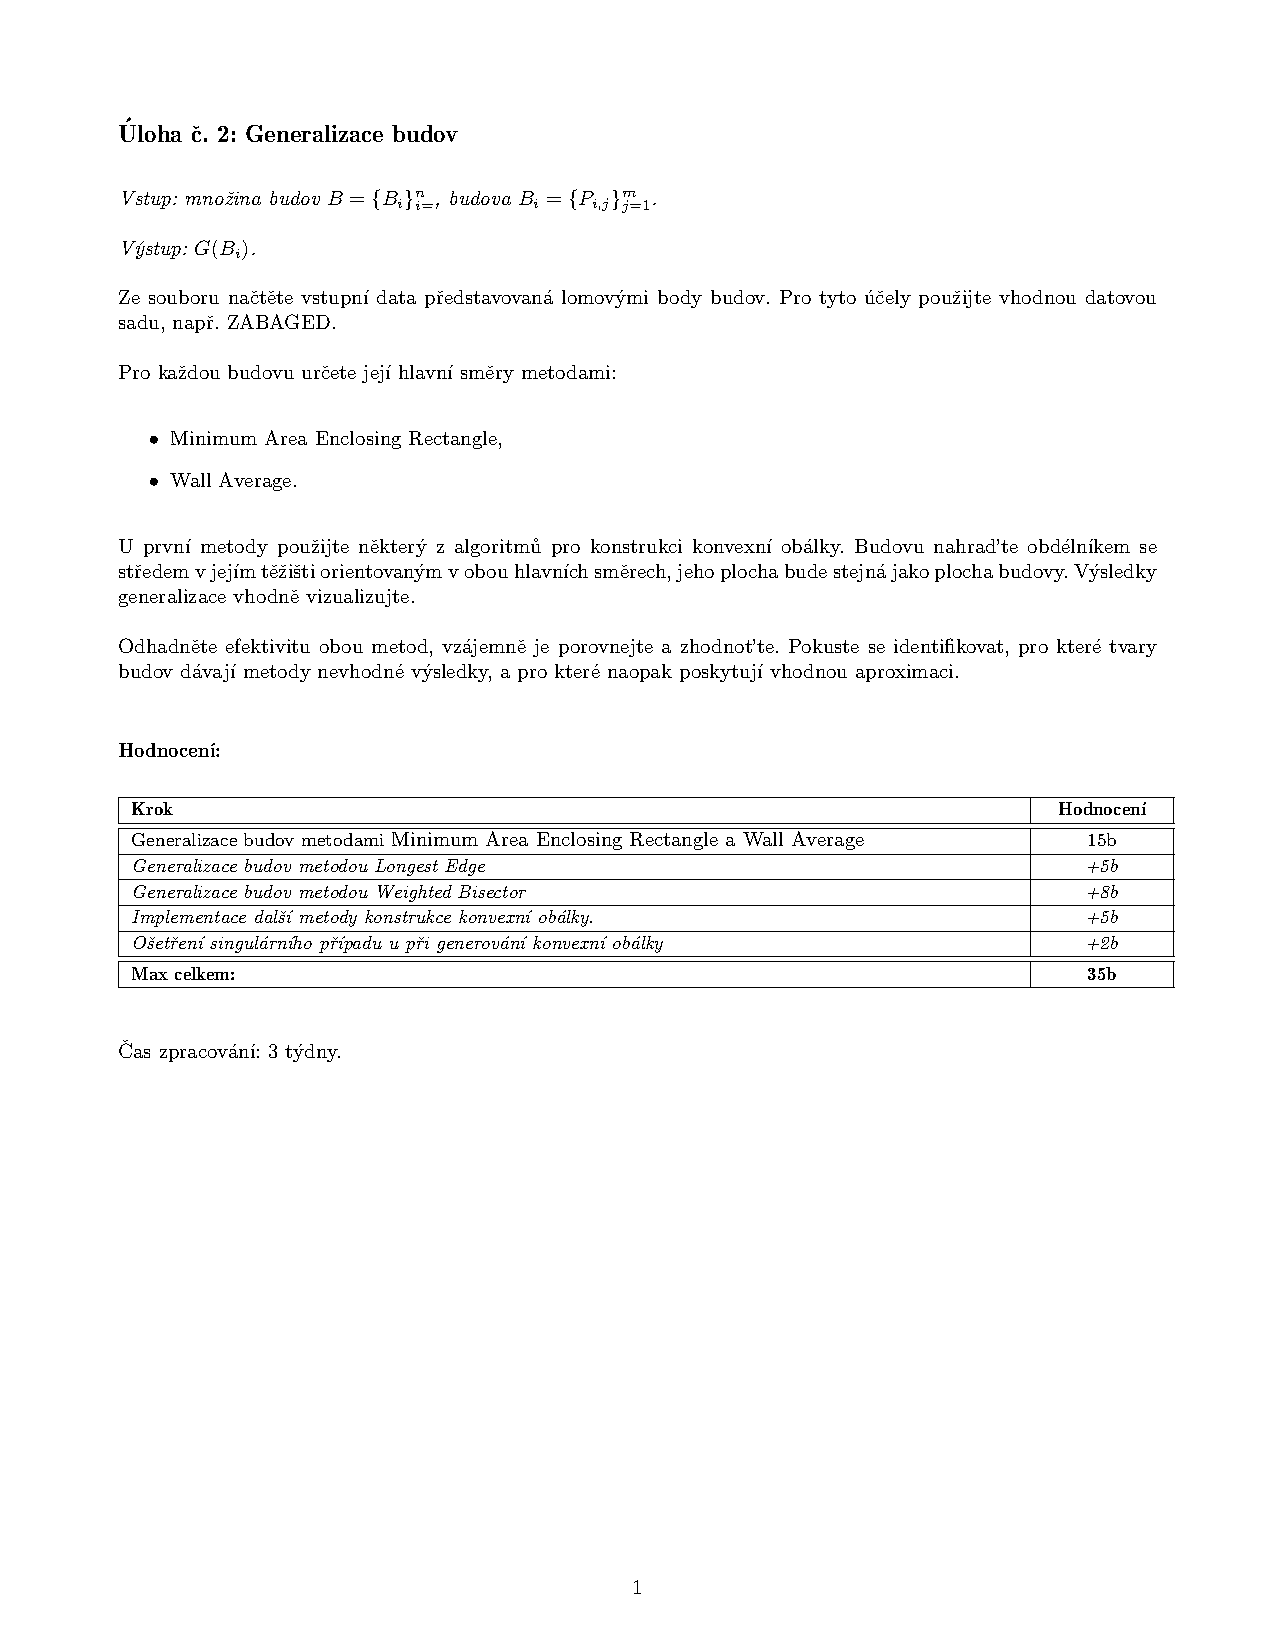
\includepdf{adkcv2}

%---------------------------------------------------------------------
\clearpage
\section{Údaje o bonusových úlohách}
\subsection{Generalizace budov metodou Longest Edge (+5b)}
Bylo implementováno určení hlavního směru metodou Longest Edge. Matematický popis algoritmu je sepsán v~kapitole~\ref{le}. Grafické znázornění fuknčního implementace algoritmu je na~obr.~\ref{fig:lon_edge}.

\subsection{Generalizace budov metodou Weighted Bisector (+8b)}
Byl implementován algoritmus Weighted Bisector, jehož popis včetně vzorců, je uveden v~kapitole~\ref{wb}. Grafické znázornění funkčnosti algoritmu je vyobrazeno na~obr.~\ref{fig:weig_bi}.

\subsection{Implementace další metody konstrukce konvexní obálky (+5b)}
Byla implementována metoda vytvoření konvexní obálky s~názvem Quick Hull. Výsledek jejího použití je na~obr.~\ref{fig:lon_edge} a obr.~\ref{fig:weig_bi}. Matematický popis řešení konstrukce konvexní obálky je součástí kapitoly~\ref{qh}.

\subsection{Ošetření singulárního případu při generování konvexní obálky (+2b)}
Tato bonusová úloha nebyla řešena.

\section{Popis a rozbor problému}
Nechť existuje libovolný polygon (tedy mnohoúhelník), který může v~praktickém případě představovat hrany budovy na mapě. Cílem této úlohy je navrhnutí několika generalizačních algoritmů, které vypočítají hlavní směr budovy a vykreslí obdélník, který však zachovává rozlohu původní budovy a platí pro něj, že jeho střed je shodný s~těžištěm budovy. Následně je vypočtena a vykreslena konvexní obálka budovy, která je určena jednou ze dvou užitých metod. Popis všech algoritmů následuje v kapitole \ref{popisalg}.

\section{Popisy algoritmů formálním jazykem} \label{popisalg}
\subsection{Minimum Area Enclosing Rectangle} \label{maer}
První hlavní směr polygonu množiny $S$ je zde představován delší ze stran minmax boxu (MMB).

\noindent\textbf{Zadáno:} Lomové body polygonu\\
\noindent\textbf{Určováno:} Hlavní směr polygonu\\
\noindent\textbf{Implementace algoritmu:}\\
\begin{enumerate}
\item Hledání konvexní obálky $H=CH(S)$,
\item inicializace obdélníku s~minimální plochou $R=MMB(S)$ a jeho plochy $A_{min}$,
\item opakování pro každou hranu $e$ obálky $H$,
\item \quad výpočet směrnice $\sigma$ hrany $e$,
\item \quad otočení $S$ o úhel $-\sigma : S_r=R(-\sigma)S$,
\item \quad nalezení $MMB(S_r)$ a určení $A(MMB(S_r))$,
\item \quad pokud $A<A_{min}$,
\item \quad \quad pak $A_{min}=A, MMB_{min}=MMB, \sigma_{min}=\sigma$,
\item $R=R(\sigma)MMB$.
\end{enumerate}

\subsection{Wall Average} \label{wa}
Na každou hranu budovy je aplikována operace $mod(\dfrac{pi}{2})$. Ze "zbytků" po dělení je vypočten vážený průměr, přičemž váhou je délka strany.

\noindent\textbf{Zadáno:} Lomové body polygonu\\ 
\noindent\textbf{Určováno:} Hlavní směr polygonu\\
\noindent\textbf{Implementace algoritmu:}\\
\begin{enumerate}
\item Určení směrnice $\sigma_0$ pro první stranu polygonu,
\item výpočet souřadnicových rozdílů $dx_i = X_{i+1}-X_{i}, dy_i=Y_{i+1}-Y_{i}$ pro sousední strany načteného polygonu,
\item určení směrnice $\sigma_i$ všech stran polygonu: $\sigma_i=atan2\dfrac{dy_i}{dx_i}$,
\item určení délek všech hran $l_i=\sqrt{dx^2+dy^2}$,
\item aplikace operace $mod(\dfrac{pi}{2})$, pro každou hranu budovy jsou redukovány směrnice: $\bigtriangleup\sigma_i=\sigma_i-\sigma^{'}$,
\item výpočet zaokrouhleného podílu: $k_i=\lfloor\frac{2\bigtriangleup\sigma_i}{pi}\rfloor$,
\item výpočet zbytku, odchylky od $0\pm k\pi : r_i=\bigtriangleup\sigma_i-k\dfrac{pi}{2}$,
\item směr natočení budovy dán váženým průměrem $\sigma=\sigma^{'}+ \sum_{i=1}^n \dfrac{r_is_i}{s_i}$.
\end{enumerate}

\subsection{Longest Edge} \label{le}
První hlavní směr budovy je představován nejdelší stranou v budově, druhý hlavní směr je na něj kolmý.

\noindent\textbf{Zadáno:} Lomové body polygonu\\
\noindent\textbf{Určováno:} Hlavní směr polygonu\\
\noindent\textbf{Implementace algoritmu:}\\
\begin{enumerate}
\item Výpočet souřadnicových rozdílů $dx_i = X_{i+1}-X_{i}, dy_i=Y_{i+1}-Y_{i}$ pro sousední strany načteného polygonu,
\item určení délek všech hran $l_i=\sqrt{dx^2+dy^2}$,
\item nalezení nejdelší hrany, pokud $l_i>l_{max}$,
\item \quad pak $l_{max}=l_i, dx_{max}=dxi, dy_{max}=dyi$,
\item směr natočení budovy: $\sigma_i=atan2\dfrac{dy_{max}}{dx_{max}}$.
\end{enumerate}


\subsection{Weighted Bisector} \label{wb}
Hledány dvě nejdelší úhlopříčky, jejich směrnice $\sigma_1, \sigma_2$ a jejich délky $s_1, s_2$. Hlavní směr~$\sigma$ je dán váženým průměrem.

\noindent\textbf{Zadáno:} Lomové body polygonu\\ 
\noindent\textbf{Určováno:} Hlavní směr polygonu\\
\noindent\textbf{Implementace algoritmu:}\\
\begin{enumerate}
\item Určení souřadnicových rozdílů pro každou úhlopříčku: $dx_{ij} = X_{j}-X_{i}, dy_{ij}=Y_{j}-Y_{i}$,
\item opakovaný výpočet délek všech úhlopříček: $s_i=\sqrt{dx^2+dy^2}$, 
\item \quad nalezení dvou nejdelších úhlopříček pokud $s_i>s_1$,
\item \quad \quad pak $s_2=s_1, s_1=s_i$ (obdobně se uloží souřadnicové rozdíly),
\item výpočet směrnice úhlopříček $s_1, s_2$: $\sigma_1=atan2\dfrac{dy_1}{dx_1}$ a $\sigma_2=atan2\dfrac{dy_2}{dx_2}$,
\item výsledné určení hlavního směru váženým průměrem: $\sigma=\dfrac{s_1\sigma_1+s_2\sigma_2}{s_1+s_2}$.
\end{enumerate}

\subsection{Jarvis Scan} \label{js}
Za předpokladu, že v~načtené množině bodů nejsou tři kolineární body, vytvoří konvexní obálku. 

\noindent\textbf{Zadáno:} Lomové body polygonu\\ 
\noindent\textbf{Určováno:} Konvexní obálka\\
\noindent\textbf{Implementace algoritmu:}\\
\begin{enumerate}
\item Nalezení pivota $q$, q$=min(y_i)$,
\item přidáni $q$ do polygonu konvexní obálky $CH$,
\item inicializace $p_{j-1}\in X, p_j=q, p_{j+1}=p_{i-1}$,
\item opakování, dokud $p_{j+1}\neq q$,
\item \quad nalezení $p_{j+1}=arg~max_{\forall p_i\in P}\angle(p_{j-1},p_j,p_i)$,
\item \quad přidání $p_{j+1}$ do konvexní obálky $CH$, 
\item \quad $p_{j-1}=p_j, p_j=p_{j+1}$.
\end{enumerate}

\subsection{Quick Hull} \label{qh}
Vytvoření konvexní obálky na základě setřídění bodů dle jejich x~--~ové souřadnice a následného rozdělení množiny bodů $S$ na horní $S_U$ a dolní část $S_L$ vzhledem k bodům s nejmenší a největší x~--~ovou souřadnicí $q_1, q_3$. Konvexní obálka $CH$ je dále konstruována ze 2 částí. Součástí algoritmu je rekurzivní volání lokální procedury Quick Hull.

\noindent\textbf{Zadáno:} Lomové body polygonu\\ 
\noindent\textbf{Určováno:} Konvexní obálka\\
\noindent\textbf{Implementace algoritmu:}\\
Globální procedura:
\begin{enumerate}
\item Nalezení bodů s minimální a maximální x~--~ovou souřadnicí $q_1=min(x_i), q_3=max(x_i)$,
\item přidání bodů $q_1, q_3$ do $S_U a S_L$,
\item pro $\forall p_i \in S$,
\item \quad pokud $(p_i\in \sigma_l(q_1,q_3))$,
\item \quad pak $p_i$ je přidán do $S_U$.
\item \quad jinak $p_i$ je přidán do $S_L$,
\item bod $q_3$ je přidán do $CH$,
\item výpočet horního segmentu $QuickHullLokalni(1,0,S_U,CH)$,
\item bod $q_1$ je přidán do $CH$,
\item výpočet dolního segmentu $QuickHullLokalni(0,1,S_L,CH)$.
\end{enumerate}

Lokální procedura:
\begin{enumerate}
\item Nalezení bodu $p^{'}=arg~max_{\forall p_i \in S}\|p_i-(p_s,p_e)\|, p^{'}\in \sigma_r(p_s,p_e)$,
\item pokud existuje bod vpravo od hrany $p^{'}\neq \emptyset$,
\item \quad pak je vypočten horní segment $QuickHullLokalni(s,i^{'},S,CH)$,
\item \quad přidání bodu $p^{'}$ do $CH$,
\item \quad výpočet dolního segmentu $QuickHullLokalni(i^{'},e,S,CH)$.
\end{enumerate}

\section{Problematické situace a jejich rozbor} \label{problemrozbor}
% (tj. simplexy) + ošetření těchto situací v kódu
Aplikace má problém při řešení algoritmu Minimum Area Enclosing Rectangle, který spočívá v~dělení nulou pro případ, jestliže jsou na vstupu dva body se stejnou x~--~ovou souřadnicí. Konkrétně se jedná o~výpočet úhlu sigma~--~viz níže (ukázka části kódu):

\begin{verbatim}
QPolygon Algorithms::minAreaEnclosingRectangle(std::vector<QPoint> &points)
{
...
        //Coordinate differences
        double dx = ch[(i+1)%n].x() - ch[i].x();
        double dy = ch[(i+1)%n].y() - ch[i].y();

        double sigma = atan2(dy, dx);
...
}
\end{verbatim}


\section{Vstupní data}
% formát vstupních dat, popis
Vstupními daty jsou souřadnice jednotlivých polygonů, které se načítají do aplikace z textového souboru. Jedná se o část budov vyexportovanou z databáze ZABAGED \cite{ZABAGED} s využitím softwaru QGIS \cite{qgis}. Polygony jsou v~souřadnicovém systém JTSK.


\section{Výstupní data}
% formát výstupních dat, popis
Za~výstup je považována grafický výstup vytvořené aplikace. Jeho součástí je implementace všech algoritmů zmíněných v~této technické zprávě. 


\section{Snímky obrazovky vytvořené aplikace a její popis}

Po~spuštění aplikace se otevře prázdné okno, do~kterého je potřeba nahrát polygony z~textového souboru a vybrat výpočetní algoritmy (obr.~\ref{fig:vyber}). Ovládání aplikace je popsáno níže. S~textem souvisí obr.~\ref{fig:popis_ui}.

\begin{enumerate}
\item \textbf{Load file with polygons}: Načtení polygonů z textového souboru. 
\item \textbf{Building simplify~--~výběr algoritmu}: Rozevírací nabídka pro volbu algoritmu určující hlavní směr budovy. 
\item \textbf{Convex Hull~--~výběr algoritmu}: Rozevírací nabídka pro volbu metody konstrukce konvexní obálky.
\item \textbf{Building simplify}: Vykreslení generalizujícího obdélníka vypočteného s~užitím zvoleného algoritmu pro určení hlavního směru budovy a vykreslení konvexní obálky.
\item \textbf{Clear added data}: Vymazání přidaných dat z~obrazovky.
\item \textbf{Clear drawing}: Vymazání ručně nakreslených polygonů.
\end{enumerate}


\begin{figure}[!htb]
	\centering
	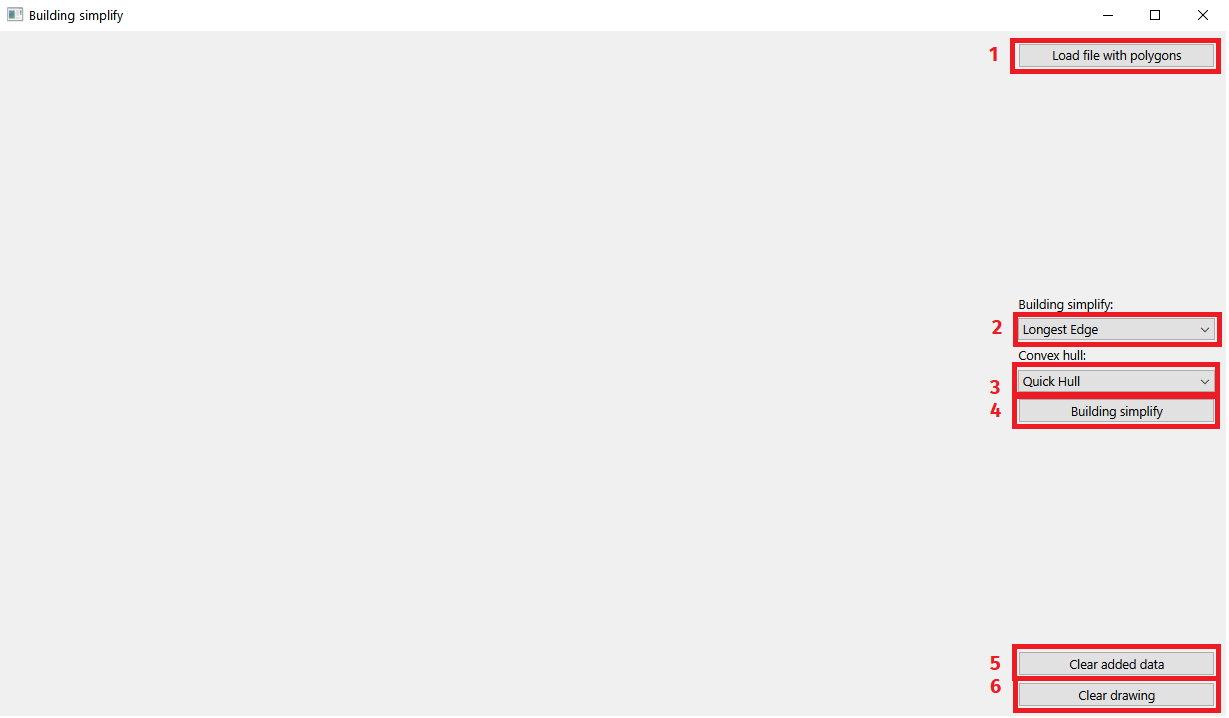
\includegraphics[scale=0.5]{obrazky/popis_ui.png} 
	\caption{Popis uživatelského rozhraní aplikace.
	}
	\label{fig:popis_ui}
\end{figure} 
\FloatBarrier

\begin{figure}[!htb]
	\centering
	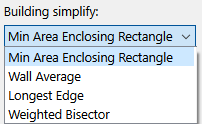
\includegraphics[scale=1]{obrazky/alg_vyber.png} 
	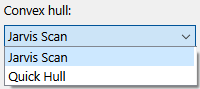
\includegraphics[scale=1]{obrazky/ch_vyber.png} 
	\caption{Ukázka rozevíracích nabídek s~algoritmy.
	}
	\label{fig:vyber}
\end{figure} 
\FloatBarrier

\textbf{Ukázka generalizace polygonů všemi použitými algoritmy (modře) s~konvexními obálkami (červeně):}
\begin{figure}[!htb]
	\centering
	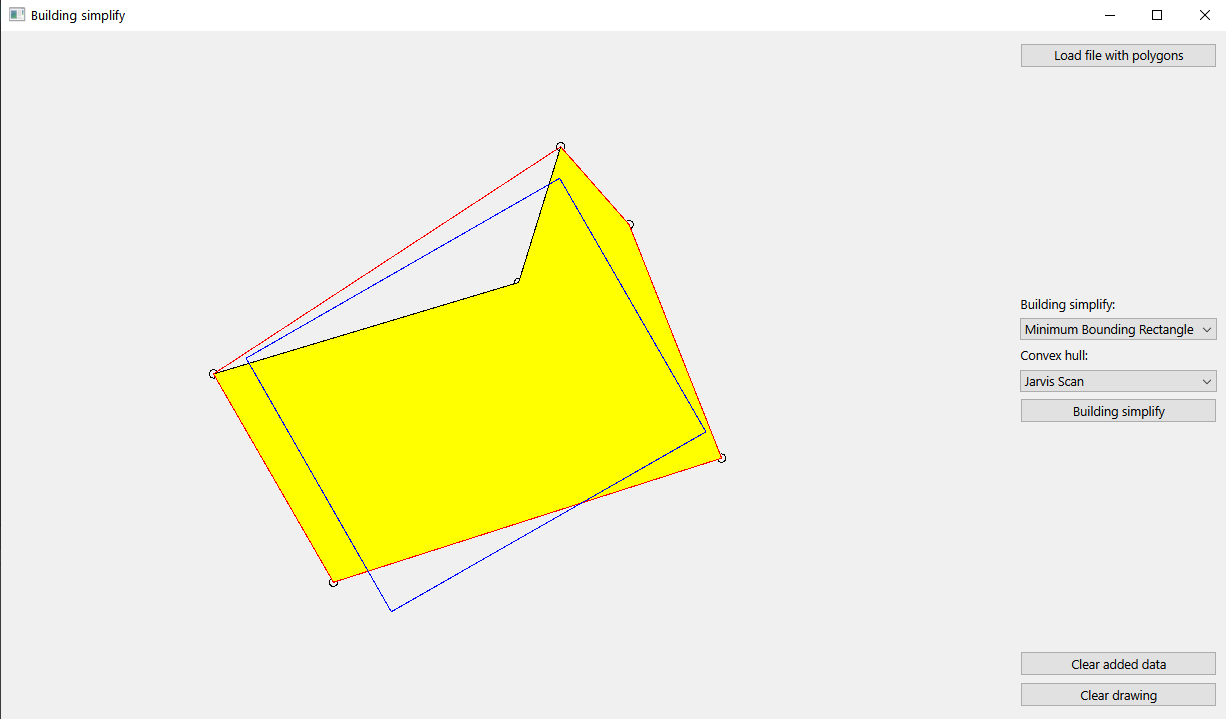
\includegraphics[scale=0.5]{obrazky/maer.png} 
	\caption{Určení hlavního směru budov s využitím algoritmu Minimum Area Enclosing Rectangle.
	}
	\label{fig:maer}
\end{figure} 
\FloatBarrier

\begin{figure}[!htb]
	\centering
	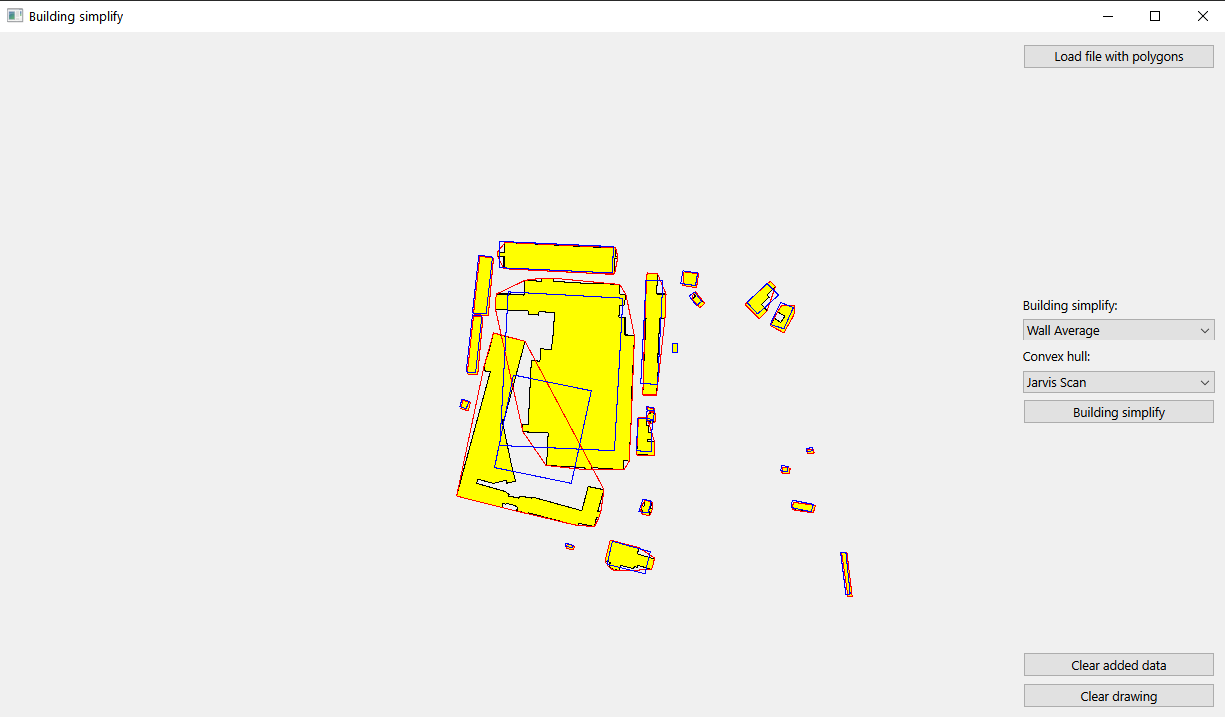
\includegraphics[scale=0.5]{obrazky/wall_avr.png} 
	\caption{Určení hlavního směru budov s využitím algoritmu Wall Average.
	}
	\label{fig:wall_avr}
\end{figure} 
\FloatBarrier

\begin{figure}[!htb]
	\centering
	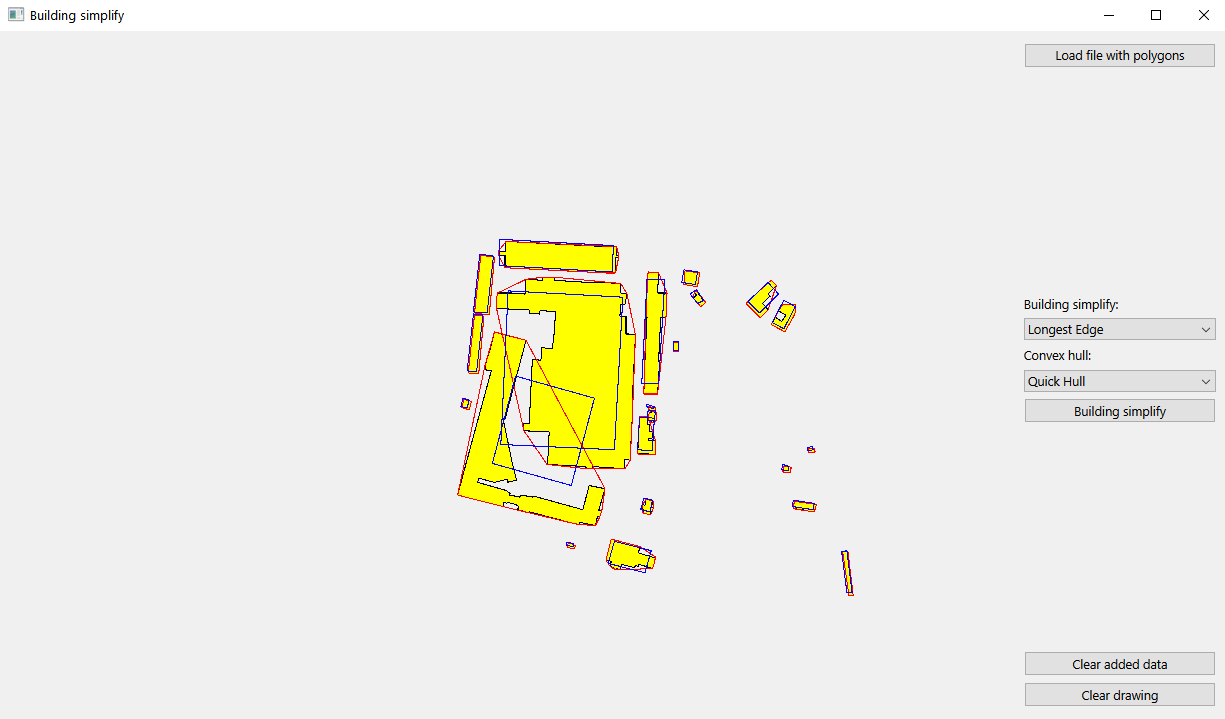
\includegraphics[scale=0.5]{obrazky/lon_edge.png} 
	\caption{Určení hlavního směru budov s využitím algoritmu Longest Edge.
	}
	\label{fig:lon_edge}
\end{figure} 
\FloatBarrier

\begin{figure}[!htb]
	\centering
	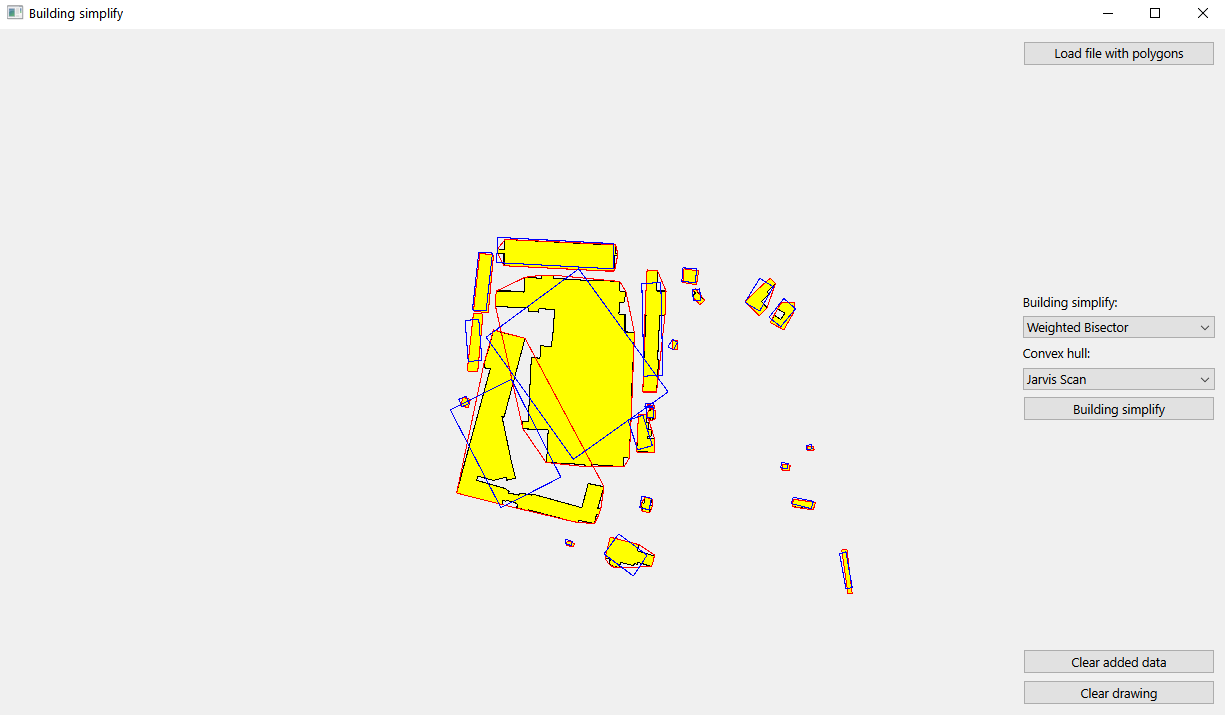
\includegraphics[scale=0.5]{obrazky/weig_bi.png} 
	\caption{Určení hlavního směru budov s využitím algoritmu Weighted Bisector.
	}
	\label{fig:weig_bi}
\end{figure} 
\FloatBarrier

\section{Dokumentace}
% popis tříd, datových položek a jednotlivých metod
\subsection{Třída Algorithms}
Tato třída obsahuje výpočetní vzorce pro použité algoritmy.

\textbf{Třída algorithms obsahuje následující veřejné metody:}

\begin{verbatim}
double get2LinesAngle(QPoint &p1, QPoint &p2, QPoint &p3, QPoint &p4)
\end{verbatim}
Metoda vypočte velikost úhlu, který svírají dvě přímky. První přímku tvoří body $p_1, p_2$ a druhou přímku body $p_3, p_4$.\\

\begin{verbatim}
int getPointLinePosition(QPoint &a,QPoint &p1,QPoint &p2)
\end{verbatim}
Metoda určuje, zda~--~li bod leží v~levé či v~pravé polorovině od přímky (hrany polygonu). Vstupními parametry jsou určovaný bod~$a$ a body $p_1, p_2$, které tvoří přímku.\\

\begin{verbatim}
double getPointLineDistance(QPoint &a, QPoint &p1, QPoint &p2)
\end{verbatim}
Metoda určuje vzdálenost bodu~$a$ od přímky tvořenou body $p_1, p_2$.\\

\begin{verbatim}
QPolygon cHullJarvisScan(std::vector <QPoint> &points)
\end{verbatim}
Výpočet konvexní obálky načtených bodů na základě algoritmu Jarvis Scan (kapitola \ref{js}).\\

\begin{verbatim}
std::vector<QPoint> rotate(std::vector<QPoint> &points, double sigma)
\end{verbatim}
Otočení načtených bodů o~zadaný úhel $sigma$.\\

\begin{verbatim}
std::tuple<std::vector<QPoint>, double> minMaxBox(std::vector<QPoint> &points)
\end{verbatim}
Proměnná vracející min~--~max box, tedy vrcholy obdélníka a jeho výměru. Vstupem jsou načtené body.\\

\begin{verbatim}
QPolygon minAreaEnclosingRectangle(std::vector<QPoint> &points)
\end{verbatim}
Určení hlavního směru polygonu s využitím algoritmu Minimum Area Eclosing Rectangle (kapitola \ref{maer}). Na vstupu jsou body polygonu. Výstupem je generalizovaný a pootočený polygon.\\

\begin{verbatim}
QPolygon wallAverage(std::vector<QPoint> &points)
\end{verbatim}
Určení hlavního směru polygonu s využitím algoritmu Wall Average (kapitola \ref{wa}). Na vstupu jsou body polygonu. Výstupem je generalizovaný a pootočený polygon.\\

\begin{verbatim}
double LH(std::vector<QPoint> &points)
\end{verbatim}
Výpočet plochy obecného mnohoúhelníků pomocí LH vzorce.\\ 

\begin{verbatim}
std::vector<QPoint> resizeRectangle(std::vector<QPoint> &points, std::vector<QPoint> &er)
\end{verbatim}
Přepočet velikosti ohraničujícího obdélníku na základě výměry původního polygonu.\\

\begin{verbatim}
QPolygon longestEdge(std::vector<QPoint> &points)
\end{verbatim}
Určení hlavního směru polygonu s využitím algoritmu Longest Edge (kapitola \ref{le}). Na vstupu jsou body polygonu. Výstupem je generalizovaný a pootočený polygon.\\

\begin{verbatim}
QPolygon weightedBisector(std::vector<QPoint> &points)
\end{verbatim}
Určení hlavního směru polygonu s využitím algoritmu Weighted Bisector (kapitola \ref{wb}). Na vstupu jsou body polygonu. Výstupem je generalizovaný a pootočený polygon.\\

\begin{verbatim}
QPolygon cHullQuickHull(std::vector <QPoint> &points)
\end{verbatim}
Výpočet konvexní obálky načtených bodů na základě algoritmu Quick Hull (kapitola \ref{qh}).\\

\begin{verbatim}
void quickHullLocal(int ps, int pe, std::vector<QPoint> &points, QPolygon &ch)
\end{verbatim}
Metoda pro pomocný výpočet rekurentního určení konvexní obálky bodů algoritmem Quick Hull, lokální procedura (kapitola \ref{qh}). Vstupními parametry jsou indexy počátečního a koncového bodu $ps$ a $pe$ vstupní hrany, načtené body a konvexní obálka.\\

    
    
\subsection{Třída Draw}
Tato třída umožňuje vykreslování bodu a polygonů.

\textbf{Třída draw obsahuje následující privátní metody a proměnné:}
\begin{verbatim}
std::vector<QPoint> points
\end{verbatim}
Proměnná se souřadnicemi načtených bodů.\\

\begin{verbatim}
QPolygon ch, er;
\end{verbatim}
Polygony pro ukládání konvexní obálky a ohraničujícího obdélníku.\\

\begin{verbatim}
std::vector<QPolygon> polygons, chs, ers
\end{verbatim}
Proměnná uchovávající pomocné polygony v~průběhu výpočtu a pro vykreslení.\\


\textbf{Třída draw obsahuje následující veřejné metody a proměnné:}
\begin{verbatim}
explicit Draw(QWidget *parent = nullptr)
\end{verbatim}
Prvotní vykreslení bodu mimo okno aplikace.\\

\begin{verbatim}
void paintEvent(QPaintEvent *event)
\end{verbatim}
Metoda, která vykresluje bod či polygony.\\

\begin{verbatim}
void mousePressEvent(QMouseEvent *event)
\end{verbatim}
Metoda určující souřadnice určeného bodu.\\

\begin{verbatim}
void clearAddedData()
\end{verbatim}
Metoda mazající přidaná data z~obrazovky.\\

\begin{verbatim}
void clearDrawing()
\end{verbatim}
Metoda mazající nakreslený polygon z~obrazovky.\\

\begin{verbatim}
std::vector<QPoint> getPoints() {return points;}
\end{verbatim}
Vrací souřadnice lomových bodů polygonu.\\

\begin{verbatim}
std::vector<QPolygon> getPolygons(){return polygons;}
\end{verbatim}
Vrací souřadnice polygonů.\\

\begin{verbatim}
void setCh(QPolygon &ch_) {chs.push_back(ch_);}
\end{verbatim}
Nastavení polygonu konvexní obálky.\\

\begin{verbatim}
void setEr(QPolygon &er_) {ers.push_back(er_);}
\end{verbatim}
Nastavení polygonu ohraničujícího obdélníku.\\

\begin{verbatim}
void clearChs(){chs.clear();}
\end{verbatim}
Smazání polygonu konvexní obálky.\\

\begin{verbatim}
void clearErs(){ers.clear();}
\end{verbatim}
Smazání polygonu ohraničujícího obdélníku.\\

\begin{verbatim}
void drawPolygons(std::vector<QPolygon> &data);
\end{verbatim}
Vykreslení polygonů načtených z~textového souboru.\\

\subsection{Třída Load}
\textbf{Třída draw obsahuje následující veřejnou proměnnou:}
\begin{verbatim}
static std::vector<QPolygon> load_file(std::string &filename)
\end{verbatim}
Umožňuje načítání polygonů z textového souboru.\\

\subsection{Třída SortByX}
\textbf{Třída draw obsahuje následující veřejnou proměnnou:}
\begin{verbatim}
bool operator() (QPoint &p1, QPoint &p2)
\end{verbatim}
Ražení bodů dle jejich x~--~ové souřadnice.\\

\subsection{Třída SortByY}
\textbf{Třída draw obsahuje následující veřejnou proměnnou:}
\begin{verbatim}
bool operator() (QPoint &p1, QPoint &p2)
\end{verbatim}
Ražení bodů dle jejich y~--~ové souřadnice.\\

\subsection{Třída Widget}
Tato třída propojuje uživatelské rozhraní aplikace s kódem. Je vytvořena v sekci \emph{Design}.

\textbf{Třída widget obsahuje následující privátní metody a proměnné:}
\begin{verbatim}
void on_pushButtonClear_clicked()
\end{verbatim}
Vymazání kresby. Propojení s~tlačítkem \emph{Clear drawing}.\\

\begin{verbatim}
void on_pushButtonLoad_clicked()
\end{verbatim}
Načtení lomových bodů polygonů z~textového souboru. Propojení s~tlačítkem \emph{Load file with polygon}.\\

\begin{verbatim}
void on_pushButton_clicked()
\end{verbatim}
Spuštění funkce Building Simplify s~vybraným algoritmem. Propojení s~tlačítkem \emph{Building Simplify}.\\

\begin{verbatim}
void on_pushButtonClearData_clicked()
\end{verbatim}
Vymazání přidaných dat. Propojení s~tlačítkem \emph{Clear added data}.\\

\begin{verbatim}
void processPoints(std::vector<QPoint> &points)
\end{verbatim}
Volba použitého algoritmu na základě výběru z~combo boxů.\\



\section{Závěr}
Byla vytvořena desktopová aplikace, která umožňuje načtení vrcholů polygonu z~textového souboru na disku. Funkcí této aplikace je vytvoření ohraničujícího polygonu, který generalizuje polygony (budovy) s~využitím jednoho ze čtyř algoritmů popsaných v~kapitole~\ref{popisalg}. Jedná se o~algoritmy Minimum Area Enclosing Rectangle, Wall Average, Longest Edge a Weighted Bisector. Ohraničující obdélník má sklon hlavního směru určený vybraným algoritmem, výměru totožnou s~původním polygonem a střed shodný s~těžištěm polygonu. Aplikace zároveň vykresluje konvexní obálku jedním ze dvou vybraných výpočtů popsaných taktéž v~kapitole~\ref{popisalg}. Těmito zvolenými výpočty jsou Jarvis Scan a Quick Hull.

\subsection{Odhad efektivity metod, vzájemné porovnání}
Nejefektivnější metodou je, z~pohledu naší skupiny, Longest Edge. Jedná se o~poměrně jednoduchý algoritmus, který sice nedosahuje nejpřesnějších výsledků, ale může sloužit jako jednoduchý generalizační nástroj například pro prvotní náhled nebo v případech, kdy není vyžadována přesnější metoda. 

Minimum Area Enclosing Rectangle se jeví jako nejproblematičtější z několika důvodů. Prvním je nutnost tvorby konvexní obálky, což není v~této úloze problém, avšak pro samostatné řešení se jedná o~překážku. Algoritmus vrací špatné výsledky pro budovy o~tvaru L~či~Z.

Nejkomplexnější metodou je, z~hlediska výpočtu, Wall Average. Tato metoda dává dobré výsledky, avšak je citlivá na polygony s~ostrými úhly. 

Weighted Bisector dává dobré výsledky, nicméně pro složitější polygony může vytvořit nežádoucí naklonění ohraničujícího obdélníku, z~důvodu výpočtu hlavního úhlu sigma přes úhlopříčky, jejichž délka a vzájemný úhel můžou být nevyzpytatelné.

\subsection{Možné či neřešené problémy} \label{mcn_problemy}
Nebyla řešena poslední bonusová úloha. Aplikace má problém při řešení algoritmu Minimum Area Enclosing Rctangle (viz \ref{problemrozbor}).

\subsection{Náměty na vylepšení} \label{vylepseni}
K~vylepšení se nabízí případ dělení nulou z~předchozí kapitoly~\ref{mcn_problemy}. Dále by bylo možné vizuálně upravit grafické prostředí aplikace. Vykreslování konvexní obálky s~užitím samostatného tlačítka bylo taktéž bráno v~potaz při psaní aplikace, avšak finální implementované řešení bylo zvoleno jako uživatelsky nejjednodušší. Zároveň by bylo možné do každé rozevírací nabídky přidat možnost nevykreslení ohraničujícího obdélníku či konvexní obálky, pokud by chtěl uživatel vykreslit pouze jednu z~možností. 


\begin{flushright}
V Praze 7.11.2021\\
\vspace{2mm}
Bc. Pane Kuzmanov\\
Bc. František Mužík\\
\end{flushright}


%---------------------------------------------------------------------
\clearpage 
\section*{Použitá literatura}
\renewcommand{\section}[2]{}%
\bibliographystyle{acm}
\bibliography{Literatura_u2_adk}


\end{document}
